\documentclass[11pt,compress,t,notes=noshow, xcolor=table]{beamer}
\usepackage[]{graphicx}\usepackage[]{color}
% maxwidth is the original width if it is less than linewidth
% otherwise use linewidth (to make sure the graphics do not exceed the margin)
\makeatletter
\def\maxwidth{ %
  \ifdim\Gin@nat@width>\linewidth
    \linewidth
  \else
    \Gin@nat@width
  \fi
}
\makeatother

\definecolor{fgcolor}{rgb}{0.345, 0.345, 0.345}
\newcommand{\hlnum}[1]{\textcolor[rgb]{0.686,0.059,0.569}{#1}}%
\newcommand{\hlstr}[1]{\textcolor[rgb]{0.192,0.494,0.8}{#1}}%
\newcommand{\hlcom}[1]{\textcolor[rgb]{0.678,0.584,0.686}{\textit{#1}}}%
\newcommand{\hlopt}[1]{\textcolor[rgb]{0,0,0}{#1}}%
\newcommand{\hlstd}[1]{\textcolor[rgb]{0.345,0.345,0.345}{#1}}%
\newcommand{\hlkwa}[1]{\textcolor[rgb]{0.161,0.373,0.58}{\textbf{#1}}}%
\newcommand{\hlkwb}[1]{\textcolor[rgb]{0.69,0.353,0.396}{#1}}%
\newcommand{\hlkwc}[1]{\textcolor[rgb]{0.333,0.667,0.333}{#1}}%
\newcommand{\hlkwd}[1]{\textcolor[rgb]{0.737,0.353,0.396}{\textbf{#1}}}%
\let\hlipl\hlkwb

\usepackage{framed}
\makeatletter
\newenvironment{kframe}{%
 \def\at@end@of@kframe{}%
 \ifinner\ifhmode%
  \def\at@end@of@kframe{\end{minipage}}%
  \begin{minipage}{\columnwidth}%
 \fi\fi%
 \def\FrameCommand##1{\hskip\@totalleftmargin \hskip-\fboxsep
 \colorbox{shadecolor}{##1}\hskip-\fboxsep
     % There is no \\@totalrightmargin, so:
     \hskip-\linewidth \hskip-\@totalleftmargin \hskip\columnwidth}%
 \MakeFramed {\advance\hsize-\width
   \@totalleftmargin\z@ \linewidth\hsize
   \@setminipage}}%
 {\par\unskip\endMakeFramed%
 \at@end@of@kframe}
\makeatother

\definecolor{shadecolor}{rgb}{.97, .97, .97}
\definecolor{messagecolor}{rgb}{0, 0, 0}
\definecolor{warningcolor}{rgb}{1, 0, 1}
\definecolor{errorcolor}{rgb}{1, 0, 0}
\newenvironment{knitrout}{}{} % an empty environment to be redefined in TeX

\usepackage{alltt}
\newcommand{\SweaveOpts}[1]{}  % do not interfere with LaTeX
\newcommand{\SweaveInput}[1]{} % because they are not real TeX commands
\newcommand{\Sexpr}[1]{}       % will only be parsed by R
\newcommand{\xmark}{\ding{55}}%


\usepackage[english]{babel}
\usepackage[utf8]{inputenc}

\usepackage{dsfont}
\usepackage{verbatim}
\usepackage{amsmath}
\usepackage{amsfonts}
\usepackage{amssymb}
\usepackage{bm}
\usepackage{csquotes}
\usepackage{multirow}
\usepackage{longtable}
\usepackage{booktabs}
\usepackage{enumerate}
\usepackage[absolute,overlay]{textpos}
\usepackage{psfrag}
\usepackage{algorithm}
\usepackage{algpseudocode}
\usepackage{eqnarray}
\usepackage{arydshln}
\usepackage{tabularx}
\usepackage{placeins}
\usepackage{tikz}
\usepackage{setspace}
\usepackage{colortbl}
\usepackage{mathtools}
\usepackage{wrapfig}
\usepackage{bm}
\usepackage{amsmath}
\usepackage{pifont}
\usepackage{xcolor} %colored math symbols

\usetikzlibrary{shapes,arrows,automata,positioning,calc,chains,trees, shadows}
\tikzset{
  %Define standard arrow tip
  >=stealth',
  %Define style for boxes
  punkt/.style={
    rectangle,
    rounded corners,
    draw=black, very thick,
    text width=6.5em,
    minimum height=2em,
    text centered},
  % Define arrow style
  pil/.style={
    ->,
    thick,
    shorten <=2pt,
    shorten >=2pt,}
}

\usepackage{subfig}

% Defines macros and environments
\usepackage{../../style/lmu-lecture}


\let\code=\texttt
\let\proglang=\textsf

\setkeys{Gin}{width=0.9\textwidth}

\setbeamertemplate{frametitle}{\expandafter\uppercase\expandafter\insertframetitle}

\usepackage{bbm}
% basic latex stuff
\newcommand{\pkg}[1]{{\fontseries{b}\selectfont #1}} %fontstyle for R packages
\newcommand{\lz}{\vspace{0.5cm}} %vertical space
\newcommand{\dlz}{\vspace{1cm}} %double vertical space
\newcommand{\oneliner}[1] % Oneliner for important statements
{\begin{block}{}\begin{center}\begin{Large}#1\end{Large}\end{center}\end{block}}


%new environments
\newenvironment{vbframe}  %frame with breaks and verbatim
{
 \begin{frame}[containsverbatim,allowframebreaks]
}
{
\end{frame}
}

\newenvironment{vframe}  %frame with verbatim without breaks (to avoid numbering one slided frames)
{
 \begin{frame}[containsverbatim]
}
{
\end{frame}
}

\newenvironment{blocki}[1]   % itemize block
{
 \begin{block}{#1}\begin{itemize}
}
{
\end{itemize}\end{block}
}

\newenvironment{fragileframe}[2]{  %fragile frame with framebreaks
\begin{frame}[allowframebreaks, fragile, environment = fragileframe]
\frametitle{#1}
#2}
{\end{frame}}


\newcommand{\myframe}[2]{  %short for frame with framebreaks
\begin{frame}[allowframebreaks]
\frametitle{#1}
#2
\end{frame}}

\newcommand{\remark}[1]{
  \textbf{Remark:} #1
}


\newenvironment{deleteframe}
{
\begingroup
\usebackgroundtemplate{
\includegraphics[width=\paperwidth,height=\paperheight]{../style/color/red.png}}
 \begin{frame}
}
{
\end{frame}
\endgroup
}
\newenvironment{simplifyframe}
{
\begingroup
\usebackgroundtemplate{
\includegraphics[width=\paperwidth,height=\paperheight]{../style/color/yellow.png}}
 \begin{frame}
}
{
\end{frame}
\endgroup
}\newenvironment{draftframe}
{
\begingroup
\usebackgroundtemplate{
\includegraphics[width=\paperwidth,height=\paperheight]{../style/color/green.jpg}}
 \begin{frame}
}
{
\end{frame}
\endgroup
}
% https://tex.stackexchange.com/a/261480: textcolor that works in mathmode
\makeatletter
\renewcommand*{\@textcolor}[3]{%
  \protect\leavevmode
  \begingroup
    \color#1{#2}#3%
  \endgroup
}
\makeatother


\input{../../latex-math/basic-math}
\input{../../latex-math/basic-ml}
\input{../../latex-math/ml-nn}

\title{Deep Learning}
\date{}

\begin{document}
\newcommand{\titlefigure}{plots/denoising_autoencoder.png}
%modify picture
\newcommand{\learninggoals}{
  \item Overcomplete AEs
  \item Sparse AEs
  \item Denoising AEs
  \item Contractive AEs
}



\lecturechapter{Regularized Autoencoders}
\lecture{I2DL}


\section{Overcomplete Autoencoders}


\begin{vbframe}{Overcomplete AE -- problem}

  Overcomplete AE (code dimension $\geq$ input dimension): even a linear AE can copy the input to the output without learning anything useful.

  \vspace{0.2cm}

  How can an overcomplete AE be useful?
 
 \vspace*{-0.3cm}
\begin{figure}[h]
    \centering
    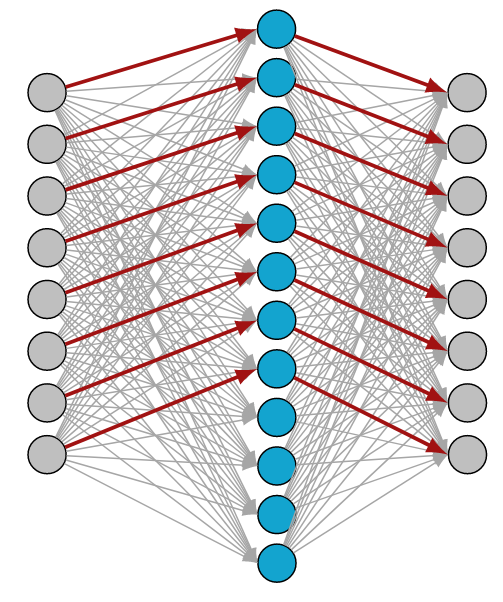
\includegraphics[width=0.35\linewidth]{plots/AE_overcomplete2.png}
    \caption{Overcomplete AE that learned to copy its inputs to the hidden layer and then to the output layer (Credits to M. Ponti).} 
\end{figure}
    
    
\end{vbframe}


% \begin{vbframe}{To powerful AE -- problem}

  
% Example 2:  Very powerful nonlinear AE that learns a 1D code:
%         \begin{itemize}
%             \item Encoder: learns to map each training example $\xv^{(i)}$ to the code $i$.
%             \item Decoder: learns to map these integer indices back to the values of specific training examples.
%         \end{itemize}
  
    
% \end{vbframe}

  \begin{frame}

  \frametitle{Regularized Autoencoder}
  
 
  %\begin{overlayarea}  
    \begin{itemize}
       \item Goal: choose code dimension and capacity of encoder/decoder based on the problem.
       \item \textbf{Regularized AEs} modify the original loss function to:
       \begin{itemize}
       \item prevent the network from trivially copying the inputs.
       \item encourage additional properties.
       \end{itemize}
       
     
       %    \pause
       %\item The model is encouraged to have additional properties
       %    \pause
        \item Examples:
            \begin{itemize}
                \item \textbf{Sparse AE:} sparsity of the representation.
               %     \pause
                \item \textbf{Denoising AE}: robustness to noise.%and outliers
             %       \pause
                \item \textbf{Contractive AE}: small derivatives of the representation w.r.t.~input.
                 %   \pause
            \end{itemize}
   
    \end{itemize} 
    $\Rightarrow$ 
    A regularized AE can be overcomplete and nonlinear but still learn something useful about the data distribution!  
  
  
\end{frame}


\section{Sparse Autoencoder}

\begin{vbframe}{Sparse Autoencoder}

\begin{itemize}
  \item \textbf{Idea:} Regularization with a sparsity constraint
  $$
    L(\xv, dec(enc(\xv))) + \lambda \|\bm{z}\|_1 
  $$
\item Try to keep the number of active neurons per training input low. 
\item Forces the model to respond to unique statistical features of the input data. 
\end{itemize}

\vspace*{-0.3cm}

\begin{figure}[h]
    \centering
    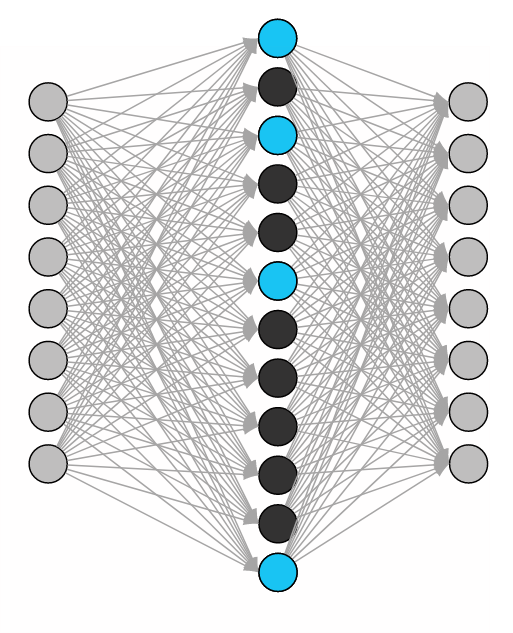
\includegraphics[width=0.25\linewidth]{plots/AE_sparse.png}
    \caption{Sparse Autoencoder (Credits to M. Ponti).} 
\end{figure}

\end{vbframe}


%\begin{vbframe}{Undercomplete Autoencoders}
%
%
%  \begin{itemize}
%    \item If our decoder is linear and the loss function the mean squared error, the undercomplete autoencoder learns to span the same subspace as principal component analysis.
%    \item Autoencoders with nonlinear encoder and nonlinear decoder functions can learn more powerful gerneralizations of PCA.
%    \item Overcomplete autoencoders without \textbf{regularization} make no sense. Even a linear encoder and linear decoder will just learn to copy the complete input layer and thus, extract no meaningful features.
%    \item[] $\Rightarrow$ we will introduce variants of \textbf{regularized} autoencoders, including \textbf{sparse} and \textbf{denoising} autoencoders.
%  \end{itemize}
%\end{vbframe}
%%%%%%%%%%%%%%%%%%%%%%%%%%%%%%%%%%%%%%%%%%%%%%%%%%%%%%%%%%%%%%%%%%
%%%%%%%%%%%%%%%%%%%%%%%%%%%%%%%%%%%%%%%%%%%%%%%%%%%%%%%%%%%%%%%%%%
%\begin{vbframe}{Sparse autoencoder}
%  \begin{itemize}
%    \item Idea: Encourage the AE
%    %he goal of a sparse autoencoder is 
%    to have as many inactive neurons in the hidden layer as possible.
%    \item That means in particular, if we use the sigmoidal activation function, we want each neuron to be
% \begin{itemize}
%       \item active, if its output is close to $1$ and
%       \item inactive, if its output is close to $0$
%     \end{itemize}
%     \item The average activation of hidden unit $j$ (over the training set) is given by $$\hat\sigma = \frac{1}{m} \displaystyle\sum_{i=1}^N (\sigma_j(x^{(i)}))$$ 
%     \item We would like to impose a \textbf{sparsity parameter} $\rho$ on the average activation of each hidden unit, such that $$\hat\sigma \leq \rho$$ 
%     \item To obtain alot of inactive units in the hidden layer, the value for $\rho$ must be set close to $0$ (e.g. $0.05$).
%        \item Add explicit regularization term 
%       %on the code $\pmb{h}$
%        to the reconstruction loss:\\
%           \begin{center}
%       $L(\xv, g(f(\xv)) + \color{red}{\lambda \Vert \frac{\partial f(\xv)}{\partial \xv} \Vert^2_F}$ 
%     \item Furthermore, we need a penalty term $\Omega(h)$ for our internal representation, that measures how distinct $\hat\sigma$ and $\rho$ are.
%     \item A common variant is the Kullback Leibler Divergence: $$KL(\rho||\hat\sigma) = \displaystyle\sum_{j=1}^{M} \rho \ log \ \frac{\rho}{\hat\sigma} + (1 - \rho) \ log \ \frac{(1 - \rho)}{(1 - \hat\sigma)}$$
%     \item Thus, our new objective evolved to $$\uauto + \Omega(h)$$
%    % \item That is equivalent to a feedforward network with regularization (chapter 2) whose task is to copy the input to the output.
%   %  \item An autoencoder that has been regularized to be sparse must respond to unique statistical features of the dataset, rather than simply acting as an identity function.
% \framebreak
%     \item One nice way to view the sparse autoencoder model is to think of a \enquote{Jack of all trades}-person.
%     \begin{itemize}
%       \item If a person is able to exert many jobs, then in general, he or she is not a master of those. On the other hand, if someone does only one or two jobs, he or she is alot more likely to be a specialist.
%       \item Similarly, if a neuron is forced to activate for any input, even if those are enormously different, then that unit will most likely not work well for all samples.
%     \end{itemize}
%     \item A typical use case for sparse autoencoders is to learn features for another objective (like classification tasks).
%   \end{itemize}
% \end{vbframe}
%%%%%%%%%%%%%%%%%%%%%%%%%%%%%%%%%%%%%%%%%%%%%%%%%%%%%%%%%%%%%%%%%%
%%%%%%%%%%%%%%%%%%%%%%%%%%%%%%%%%%%%%%%%%%%%%%%%%%%%%%%%%%%%%%%%%%

\section{Denoising Autoencoders}

\begin{vbframe}{Denoising autoencoders (DAE)}

The denoising autoencoder (DAE) is an autoencoder that receives a corrupted data point as input and is trained to predict the original, uncorrupted data point as its output.

    \begin{itemize}
       \item Idea: representation should be robust to introduction of noise.
       \item Produce corrupted version $\tilde{\xv} $ of  input $\xv$, e.g.~by
     \begin{itemize}  
        \item random assignment of subset of inputs to 0.
      \item adding Gaussian noise.
       \end{itemize}
        %\item 
        \item Modified reconstruction loss: $L(\xv, \color{red}{dec(enc(\tilde{\xv}))}\color{black}{)}$ \\ %instead of $L(\xv, g(f(\xv))$   
            %\begin{itemize}
            %\item $\tilde{\xv}$ is a copy of $\xv$ corrupted with some form of noise\\
           % \end{itemize}
           $\rightarrow$ denoising AEs must learn to undo this corruption.
         %   $\Rightarrow$ $f$ and $g$ implicitly learn the structure of $p_{data}(\xv)$
    \end{itemize}
  
\framebreak

  \begin{itemize}
   % \item A denoising autoencoder minimizes $$\dauto$$ where $\tilde{x}$ is a copy of x, which has been corrupted by noise.
    \item %Denoising autoencoders must therefore undo this corruption rather than simply copying their input. Training forces f and g to implicitly learn the structure of $p_{data}(x)$. 
    %The stochastic corruption process turns the DAE into a stochastic AE.
    With the  corruption process, we induce stochasticity  into the DAE.
    \item Formally: let $C(\tilde{\xv}|\xv)$ present the conditional distribution of corrupted samples $\tilde{\xv}$, given a data sample $\xv$.
    \item  Like feedforward NNs can model a distribution over targets $p(\mathbf{y}|\xv)$, output units and loss function of an AE can be chosen such that one gets a stochastic decoder $p_{decoder}(\xv|\mathbf{z})$.
    \item E.g.~linear output units to parametrize the mean of Gaussian distribution for real valued $\xv$ and negative log-likelihood loss (which is equal to MSE).
    \item The DAE then learns a  reconstruction distribution $p_{reconstruct}(\xv|\tilde{\xv})$ from training pairs $(\xv, \tilde{\xv})$.
  \item (Note that the encoder could also be made stochastic, modelling $p_{encoder}(\mathbf{z}|\tilde{\xv})$.)
  \end{itemize}
\framebreak
  The general structure of a DAE as a computational graph:
  \begin{figure}
    \centering
    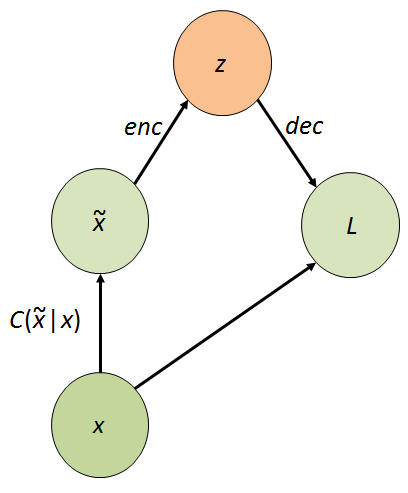
\includegraphics[width=4.5cm]{plots/denoising_autoencoder_basic_structure.png}
    \caption{Denoising autoencoder: \enquote{making the learned representation
robust to partial corruption of the input pattern.}}
  \end{figure}
%\framebreak
%  \begin{algorithm}[H]
%    \caption{Training denoising autoencoders}
%    \begin{algorithmic}[1]
%    \State Sample a training example $\xv$ from the training data.
%    \State Sample a corrupted version $\tilde{\xv}$ from $C(\tilde{\xv}|\xv)$
%    \State \parbox[t]{\dimexpr\linewidth-\algorithmicindent}{Use $(\xv, \tilde{\xv})$ as a training example for estimating the AE reconstruction $p_{reconstruct}(\xv|\tilde{\xv}) = p_{decoder}(\xv|\mathbf{z})$, where \\ 
%    - $\mathbf{z}$ is the output of the encoder $enc(\tilde{\xv})$ and \\
%    - $p_{decoder}$ defined by a decoder $dec(\mathbf{z})$}
%    \end{algorithmic}
%  \end{algorithm}
%  \begin{itemize}
%   \item All we have to do to transform an AE into a DAE is to add a stochastic corruption process on the input.
%    \item The DAE still tries to preserve the information about the input (encode it), but also to undo the effect of a corruption process!
%  \end{itemize} 
\framebreak
  \begin{figure}
    \centering
    % 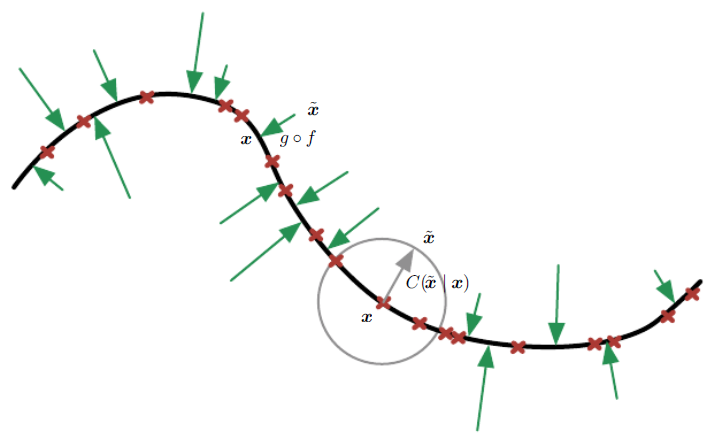
\includegraphics[width=4.5cm]{plots/denoising_autoencoder.png}
    \scalebox{0.7}{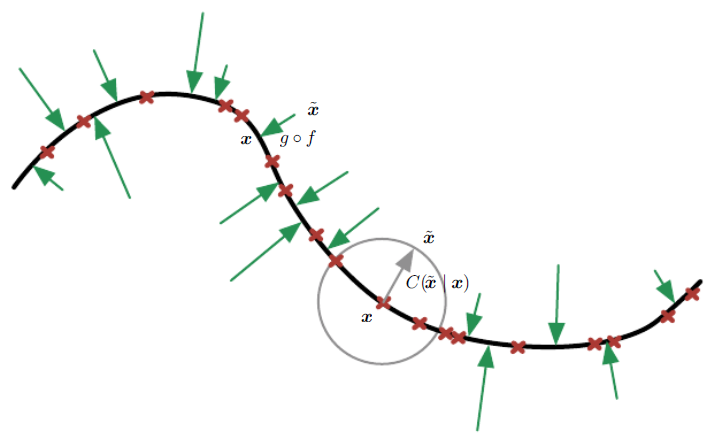
\includegraphics{plots/denoising_autoencoder.png}}
    \caption{Denoising autoencoders - \enquote{manifold perspective} (Ian Goodfellow et al. (2016))}
  \end{figure}
    A DAE is trained to map a corrupted data point $\tilde{\xv}$ back to
the original data point $\xv$.
  \framebreak
\begin{figure}
    \centering
    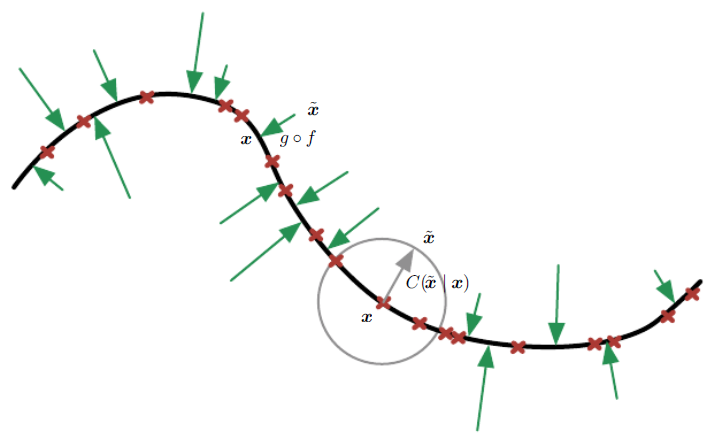
\includegraphics[width=4.5cm]{plots/denoising_autoencoder.png}
    % \scalebox{0.7}{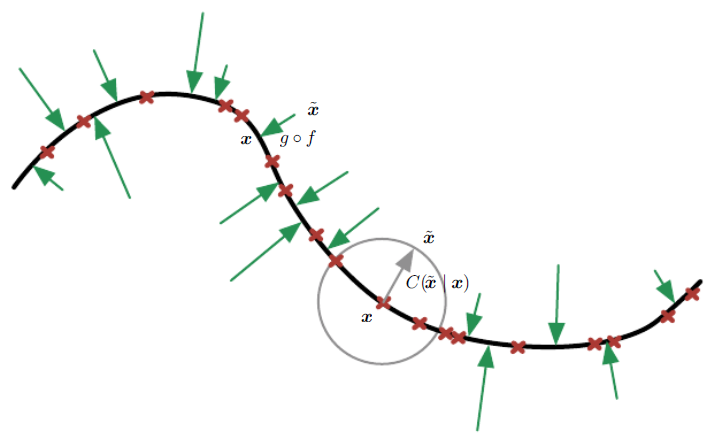
\includegraphics{plots/denoising_autoencoder.png}}
    \caption{Denoising autoencoders - \enquote{manifold perspective} (Ian Goodfellow et al. (2016))}
  \end{figure}
  \begin{itemize}
    \item The corruption process $C(\tilde{\xv}|\xv)$ is displayed by the gray circle of equiprobable corruptions
    \item Training a DAE  by minimizing  $||dec(enc(\tilde{\xv})) - \xv||^2$ corresponds to minimizing $
    \mathbb{E}_{\xv,\tilde{\xv}\sim p_{data}(\xv)C(\tilde{\xv}|\xv)}[- \log p_{decoder}(\xv|f(\tilde{\xv}))]$.
  \end{itemize}
\framebreak
\begin{figure}
    \centering
    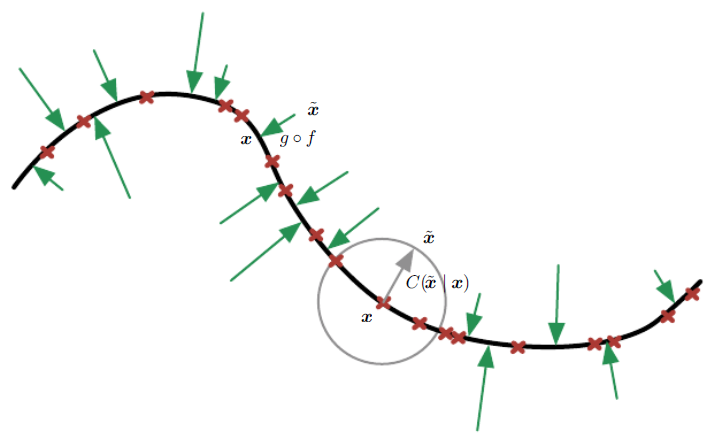
\includegraphics[width=4.5cm]{plots/denoising_autoencoder.png}
    \caption{Denoising autoencoders - \enquote{manifold perspective} (Ian Goodfellow et al. (2016))}
  \end{figure}
  \begin{itemize}
 
    \item The vector $dec(enc(\tilde{\xv})) - \tilde{\xv}$ points approximately towards the nearest point in the  data manifold, since $dec(enc(\tilde{\xv}))$ estimates the center of mass of clean points $\xv$ which could have given rise to $\tilde{\xv}$.
    \item Thus, the DAE learns a vector field $dec(enc(\tilde\xv)) - \xv$ indicated by the green arrows.
  \end{itemize}
  
\framebreak

An example of a vector field learned by a DAE. 
  
  \begin{figure}
    \centering
    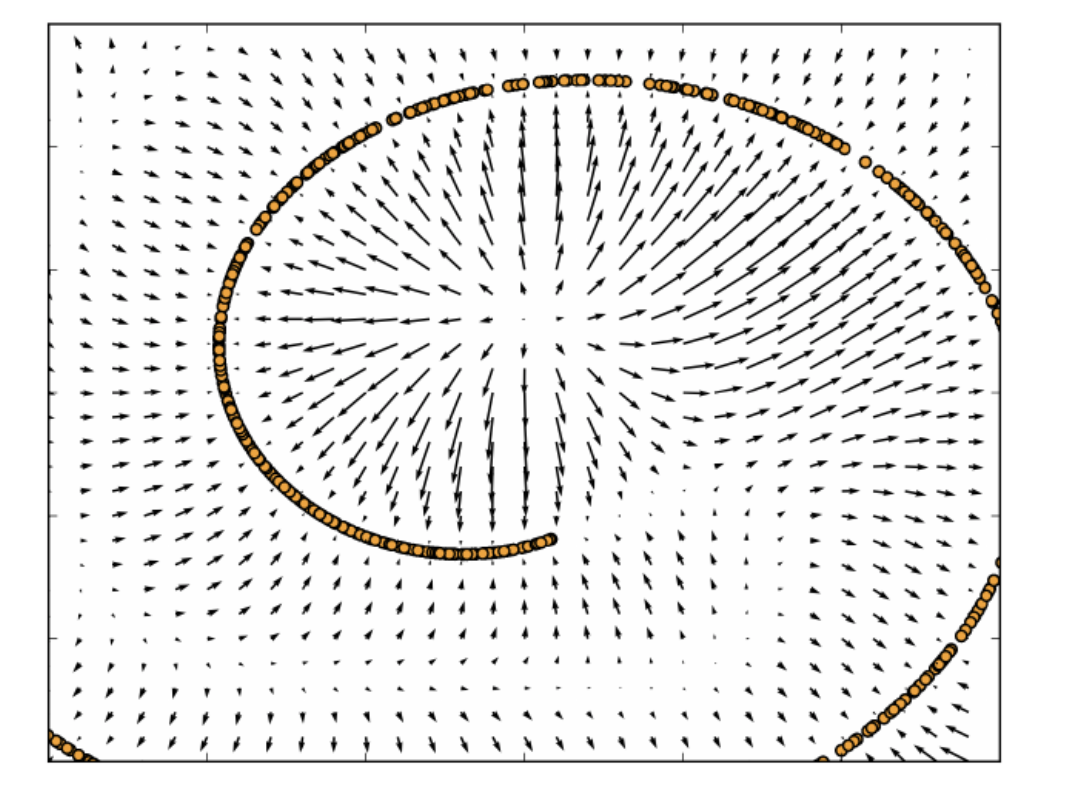
\includegraphics[width=4.5cm]{plots/DAE-vectorfield.png}
    \caption{ source: Ian Goodfellow et al. (2016)}
  \end{figure}
  
  
\end{vbframe}
%%%%%%%%%%%%%%%%%%%%%%%%%%%%%%%%%%%%%%%%%%%%%%%%%%%%%%%%%%%%%%%%%%
%%%%%%%%%%%%%%%%%%%%%%%%%%%%%%%%%%%%%%%%%%%%%%%%%%%%%%%%%%%%%%%%%%
\begin{frame}{Experiment: Encode MNIST with a DAE}
  \begin{itemize}
    \item We will now corrupt the MNIST data with Gaussian noise and then try to denoise it as good as possible.
  \end{itemize}
  \begin{figure}
    \centering
    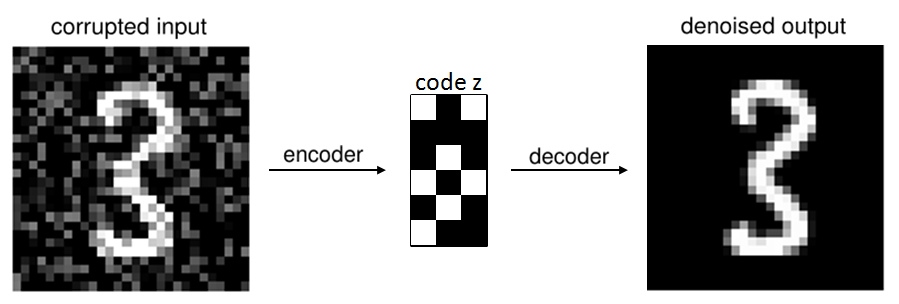
\includegraphics[width=11cm]{plots/denoised_autoencoder_mnist_problem.png}
    \caption{Flow chart of our autoencoder: denoise the corrupted input.}
  \end{figure}  
\end{frame}
%%%%%%%%%%%%%%%%%%%%%%%%%%%%%%%%%%%%%%%%%%%%%%%%%%%%%%%%%%%%%%%%%%
%%%%%%%%%%%%%%%%%%%%%%%%%%%%%%%%%%%%%%%%%%%%%%%%%%%%%%%%%%%%%%%%%%
\begin{frame}{Experiment: Encode MNIST with a DAE}
  \begin{itemize}
    \item To corrupt the input, we randomly add or subtract values from a uniform distribution to each of the image entries.
  \end{itemize}
  \begin{figure}
    \centering
    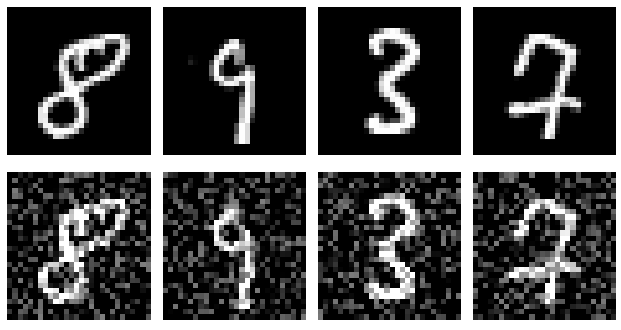
\includegraphics[width=9cm]{plots/mnist_noise.png}
    \caption{Top row: original data, bottom row: corrupted mnist data.}
  \end{figure}
\end{frame}

%%%%%%%%%%%%%%%%%%%%%%%%%%%%%%%%%%%%%%%%%%%%%%%%%%%%%%%%%%%%%%%%%%
%%%%%%%%%%%%%%%%%%%%%%%%%%%%%%%%%%%%%%%%%%%%%%%%%%%%%%%%%%%%%%%%%%
\frame{

\frametitle{Experiment: Encode MNIST with a DAE}
  
  \center
  \begin{figure}

    \only<1>{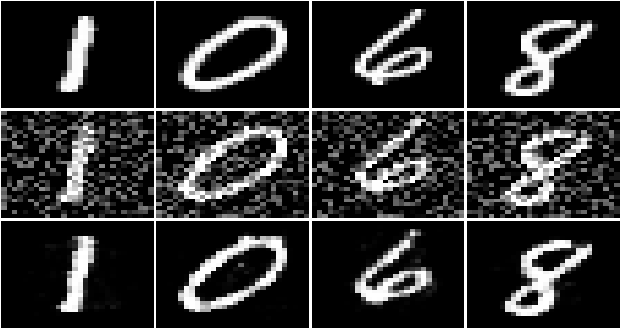
\includegraphics[width=10.7cm]{plots/denoised_1568_2.png}}%  
    \only<2>{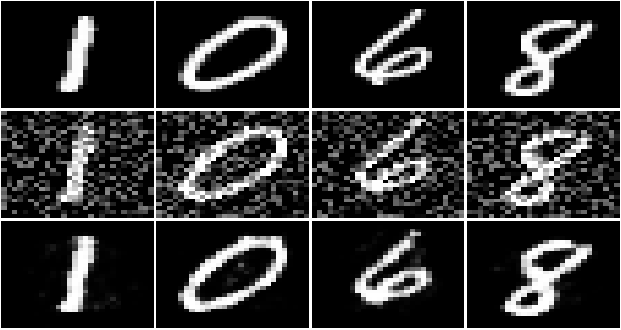
\includegraphics[width=10.7cm]{plots/denoised_784_2.png}}%
    \only<3>{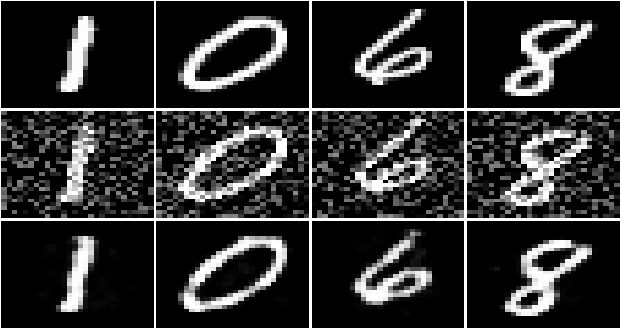
\includegraphics[width=10.7cm]{plots/denoised_256_2.png}}%
    \only<4>{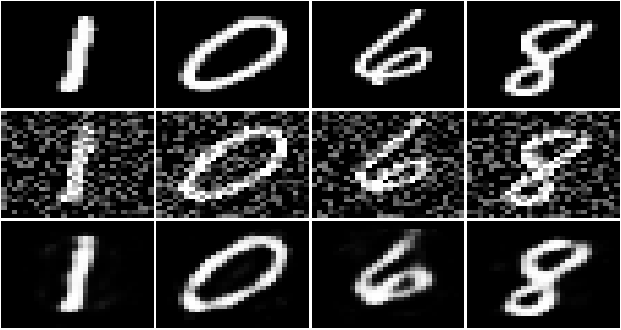
\includegraphics[width=10.7cm]{plots/denoised_64_2.png}}%
    \only<5>{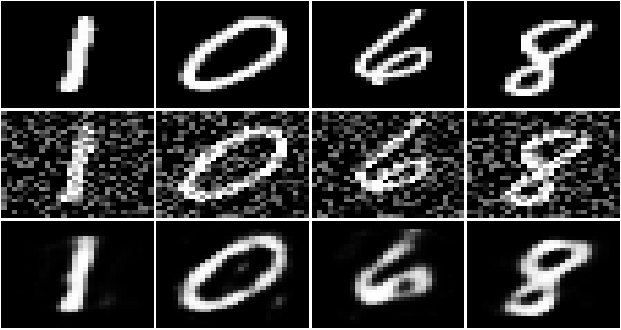
\includegraphics[width=10.7cm]{plots/denoised_32_2.png}}%
    \only<6>{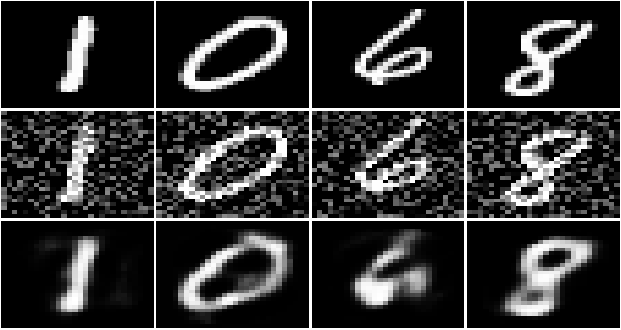
\includegraphics[width=10.7cm]{plots/denoised_16_2.png}}%
    \only<7>{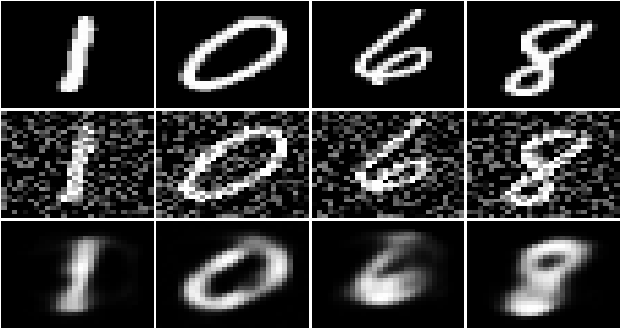
\includegraphics[width=10.7cm]{plots/denoised_8_2.png}}%
    \caption{The top row shows the original digits, the intermediate one the corrupted and the bottom row the denoised/reconstructed digits (prediction).}
    
  \end{figure}
  
  \vspace{-0.3cm}
  
  \begin{itemize}
  
 \only<1>{\item $dim(\pmb{z}) = 1568$ (overcomplete).}
    \only<2>{\item $dim(\pmb{z}) = 784$ ($= dim(\xv)$).}
    \only<3>{\item $dim(\pmb{z}) = 256$.}
    \only<4>{\item $dim(\pmb{z}) = 64$.}
    \only<5>{\item $dim(\pmb{z}) = 32$.}
    \only<6>{\item $dim(\pmb{z}) = 16$.}
    \only<7>{\item $dim(\pmb{z}) = 8$.}
    
  \end{itemize}
  
}
%%%%%%%%%%%%%%%%%%%%%%%%%%%%%%%%%%%%%%%%%%%%%%%%%%%%%%%%%%%%%%%%%%
%%%%%%%%%%%%%%%%%%%%%%%%%%%%%%%%%%%%%%%%%%%%%%%%%%%%%%%%%%%%%%%%%%
% \frame{

% \frametitle{Experiment: Encode MNIST with a DAE}
% 
%   \begin{itemize}
%   
%     \only<1>{\item Let us increase the amount of noise and see how the autoencoder with $dim(z) = 64$ deals with it (for science!).}
%     \only<2>{\item A lot of noise.}
%     \only<3>{\item \textbf{A lot} of noise.}
%     
%   \end{itemize}
%   
%   \center
%   \begin{figure}
% 
%     \only<2>{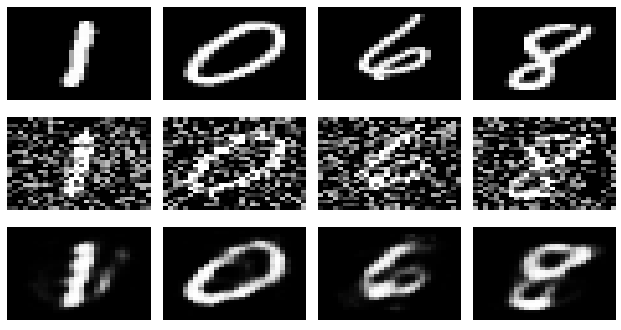
\includegraphics[width=10.7cm]{plots/denoised_alot_64.png}}%  
%     \only<3>{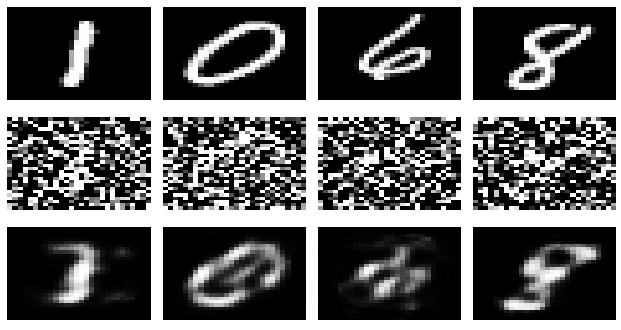
\includegraphics[width=10.7cm]{plots/denoised_alot2_64.png}}%
%     
%   \end{figure}
%   
% }

\section{Contractive Autoencoder}

\begin{frame}[t]{Contractive Autoencoder}
   \begin{itemize}
      \item Goal: For very similar inputs, the learned encoding should also be very similar. 
      \item We can train our model in order for this to be the case by requiring that the \textbf{derivative of the hidden layer activations are small} with respect to the input. 
      \item In other words: The encoded state $enc(\xv)$ should not change much for small changes in the input. 
      \item Add explicit regularization term to the reconstruction loss:\\
           \begin{center}
       $L(\xv, dec(enc(\xv)) + \color{red}{\lambda \Vert \frac{\partial enc(\xv)}{\partial \xv} \Vert^2_F}$ 
   \end{center}
% %        \pause
%   $\Rightarrow$  Derivatives of the encoder function w.r.t.~the input are encouraged to be small. \\
% %        \pause
%     $\Rightarrow$ Only a small number of input directions will have significant derivatives.\\ 
% %        \pause
%   $\Rightarrow$ The encoder function is encouraged to resist infinitesimal perturbations of the input.
   \end{itemize} 

\end{frame}


\begin{frame}[t]{DAE vs. CAE}
    \begin{table}[h!]
        \centering
        \label{tab:}
        \begin{tabular}{p{5cm}|p{5cm}}
            \textbf{DAE} & \textbf{CAE}\\
            \hline
%            \pause
            the \textit{decoder} function is trained to resist infinitesimal perturbations of the input. & the \textit{encoder} function is trained to resist infinitesimal perturbations of the input.
        \end{tabular}
    \end{table}

\begin{itemize}
\item Both the denoising and contractive autoencoders perform well.
\item Advantage of denoising autoencoder: simpler to implement
\begin{itemize}
\item  requires adding one or two lines of code to regular AE.
\item  no need to compute Jacobian of hidden layer.
\end{itemize}
\item Advantage of contractive autoencoder: gradient is deterministic
\begin{itemize}
\item can use second order optimizers (conjugate gradient, LBFGS, etc.).
\item might be more stable than the denoising autoencoder, which uses a sampled gradient.
\end{itemize}

\end{itemize}

\end{frame}

\begin{vbframe}
\frametitle{References}
\footnotesize{
\begin{thebibliography}{99}
%%%%%%%%%%%%%%%%%%%%%%%%%%%%%%%%%%
\bibitem[Ian Goodfellow et al., 2016]{1} Ian Goodfellow, Yoshua Bengio and Aaron Courville (2016)
\newblock Deep Learning
\newblock \emph{\url{http://www.deeplearningbook.org/}}

\bibitem[M. Ponti et al., 2016]{1} Everything you wanted to know about Deep Learning for Computer Vision but were afraid to ask (2017)
\newblock SIBGRAPI Tutorials 2017
%%%%%%%%%%%%%%%%%%%%%%%%%%%%%%%%%%

\end{thebibliography}
}
\end{vbframe}


\endlecture
\end{document}
